\documentclass{beamer}
\usepackage{pdfpages}
\usepackage{graphicx}

% Remove navigation symbols
\setbeamertemplate{navigation symbols}{}

\title{Curse of Dimensionality}

\begin{document}

% \frame{\titlepage}

\begin{frame}{Overview}

\textbf{Source: } \url{https://slds-lmu.github.io/i2ml/chapters/14_cod/}

\begin{itemize}
    \item How our intuitions miserably fails as the dimensionality of the data increases
    \item Properties of high dimensional data
    \item Implications for distance based algorithms (e. g. KMeans, kNN)
    \item How to deal with those implications
    \item Most importantly - what happens if we peel a high dimensional mandarin (we will also have a practical session for the 3D case)
\end{itemize}
\end{frame}


\section{The Curse}
\includepdf[pages=2-18,scale=1.3,offset=50 -10]{slides-cod.pdf}

\begin{frame}{Gaussian soap bubble: where is the typical sample?}

Consider $X \sim \mathcal{N}(0, I_p)$ in $p$ dimensions.

\begin{itemize}
    \item The \emph{mode} (densest point) is at the origin.
    \item \textbf{Question:} where do typical samples actually land?
\end{itemize}

\pause

\vspace{0.5em}
The squared norm $\|X\|^2 \sim \chi^2_p$, so
\[
    \mathbb{E}\|X\| \approx \sqrt{p}, \qquad \operatorname{std}(\|X\|) \to \text{const as } p \to \infty.
\]

Typical samples sit on a thin shell at radius $\sqrt{p}$. The densest point is the \emph{least likely} place to draw from.

\vspace{0.5em}
\textbf{Why this matters:} foundation for MCMC initialization, diffusion-model noise schedules, and the "soap bubble" picture of high-dim Gaussians. The mode of a distribution is \emph{not} where its mass lives.

\end{frame}

\section{ML Examples}
\includepdf[pages=2-last,scale=1.3,offset=50 -10]{slides-cod-examples.pdf}

\begin{frame}{Hughes peaking: more features can hurt}

\textbf{Setup:} fix training set size $n$. Vary number of features $p$. Train a classifier and measure accuracy.

\vspace{0.5em}
\textbf{Predict:} how does accuracy depend on $p$?

\pause

\begin{itemize}
    \item Accuracy rises with $p$ (more information).
    \item Then it \textbf{peaks}.
    \item Then it \emph{degrades} -- even though we keep adding "information."
\end{itemize}

\vspace{0.5em}
This is the \emph{Hughes phenomenon} (1968). The Boston Housing + noise features experiment was exactly this.

\vspace{0.5em}
\textbf{Takeaway:} throwing away features can improve accuracy. The optimal $p$ depends on $n$ and the signal-to-noise ratio of each feature. This is why feature selection is not optional.

\end{frame}

\section{Pop Quiz}
\begin{frame}
    Why do we use cosine similarity instead of the Euclidean distance?
\end{frame}

\begin{frame}{Why do we use cosine similarity? (answer)}

\textbf{The puzzle:} in high dimensions, Euclidean distances collapse together (we saw this for k-NN). So how can any distance-based method work?

\pause

\vspace{0.5em}
\textbf{Key insight:} distances concentrate, but \emph{angles} still discriminate.

\begin{itemize}
    \item Radial coordinate $\|x\|$ concentrates around $\sqrt{p}$ -- noisy, uninformative.
    \item Direction $x / \|x\|$ keeps the signal.
\end{itemize}

\vspace{0.5em}
For unit vectors $x, y$:
\[
    \cos(\theta) = 1 - \tfrac{1}{2} \|x - y\|^2.
\]

Same information in principle -- but cosine ignores the concentrated radius. For TF-IDF and word/sentence embeddings: document length is irrelevant, word-direction carries the meaning.

\end{frame}

\section{The Blessing Side}

\begin{frame}{Random vectors are (almost) orthogonal}

Draw two vectors uniformly from the unit sphere $S^{p-1}$. What is the angle between them?

\pause

\vspace{0.5em}
The angle concentrates at $90^\circ$, with standard deviation $\approx 1/\sqrt{p}$.

\vspace{0.5em}
\textbf{Stronger statement:} you can pack $e^{c \cdot p}$ \emph{almost-orthogonal} vectors into $\mathbb{R}^p$ (pairwise $|\langle u, v \rangle| < \epsilon$). Compare to only $p$ truly orthogonal vectors.

\vspace{0.5em}
\textbf{Why this matters -- LLM superposition:} GPT-style models use embeddings of dimension $d \approx 12{,}288$. They store millions of "concepts" by exploiting near-orthogonality -- many more concepts than the embedding dimension, with minimal interference between them.

\vspace{0.5em}
The curse becomes a \emph{feature}.

\end{frame}

\section{Why Deep Learning Escapes the Curse}

\begin{frame}{The manifold hypothesis}

A $256 \times 256$ RGB image lives in $\mathbb{R}^{196{,}608}$. But the set of "natural images" -- photos of faces, of Yerevan streets, of cats -- is a vanishingly thin \emph{manifold} of effective dimension maybe a few thousand.

\vspace{0.5em}
\textbf{Same for:}
\begin{itemize}
    \item Sentences (vs. random character strings)
    \item Audio of speech (vs. white noise)
    \item Gene expression patterns of real cells (vs. arbitrary $\mathbb{R}^{20000}$ vectors)
\end{itemize}

\vspace{0.5em}
\textbf{The curse is real} for arbitrary high-dim data. \textbf{Real data is structured.} Deep networks learn the manifold instead of the ambient space -- that is why they work where k-NN dies.

\vspace{0.5em}
\emph{Bridge to representation learning: the next chapter.}

\end{frame}


\end{document}